\documentclass[border=1pt]{standalone}
\usepackage[dvipsnames]{xcolor}
\usepackage{tikz}                       % Graphen und kommutative Diagramme
\usetikzlibrary{patterns}               % Um schraffierte Formen in der tikzpicture-Umgebung zu zeichnen.

\begin{document}

\newcommand{\ul}{\underline}

\centering
\resizebox{!}{8cm}{
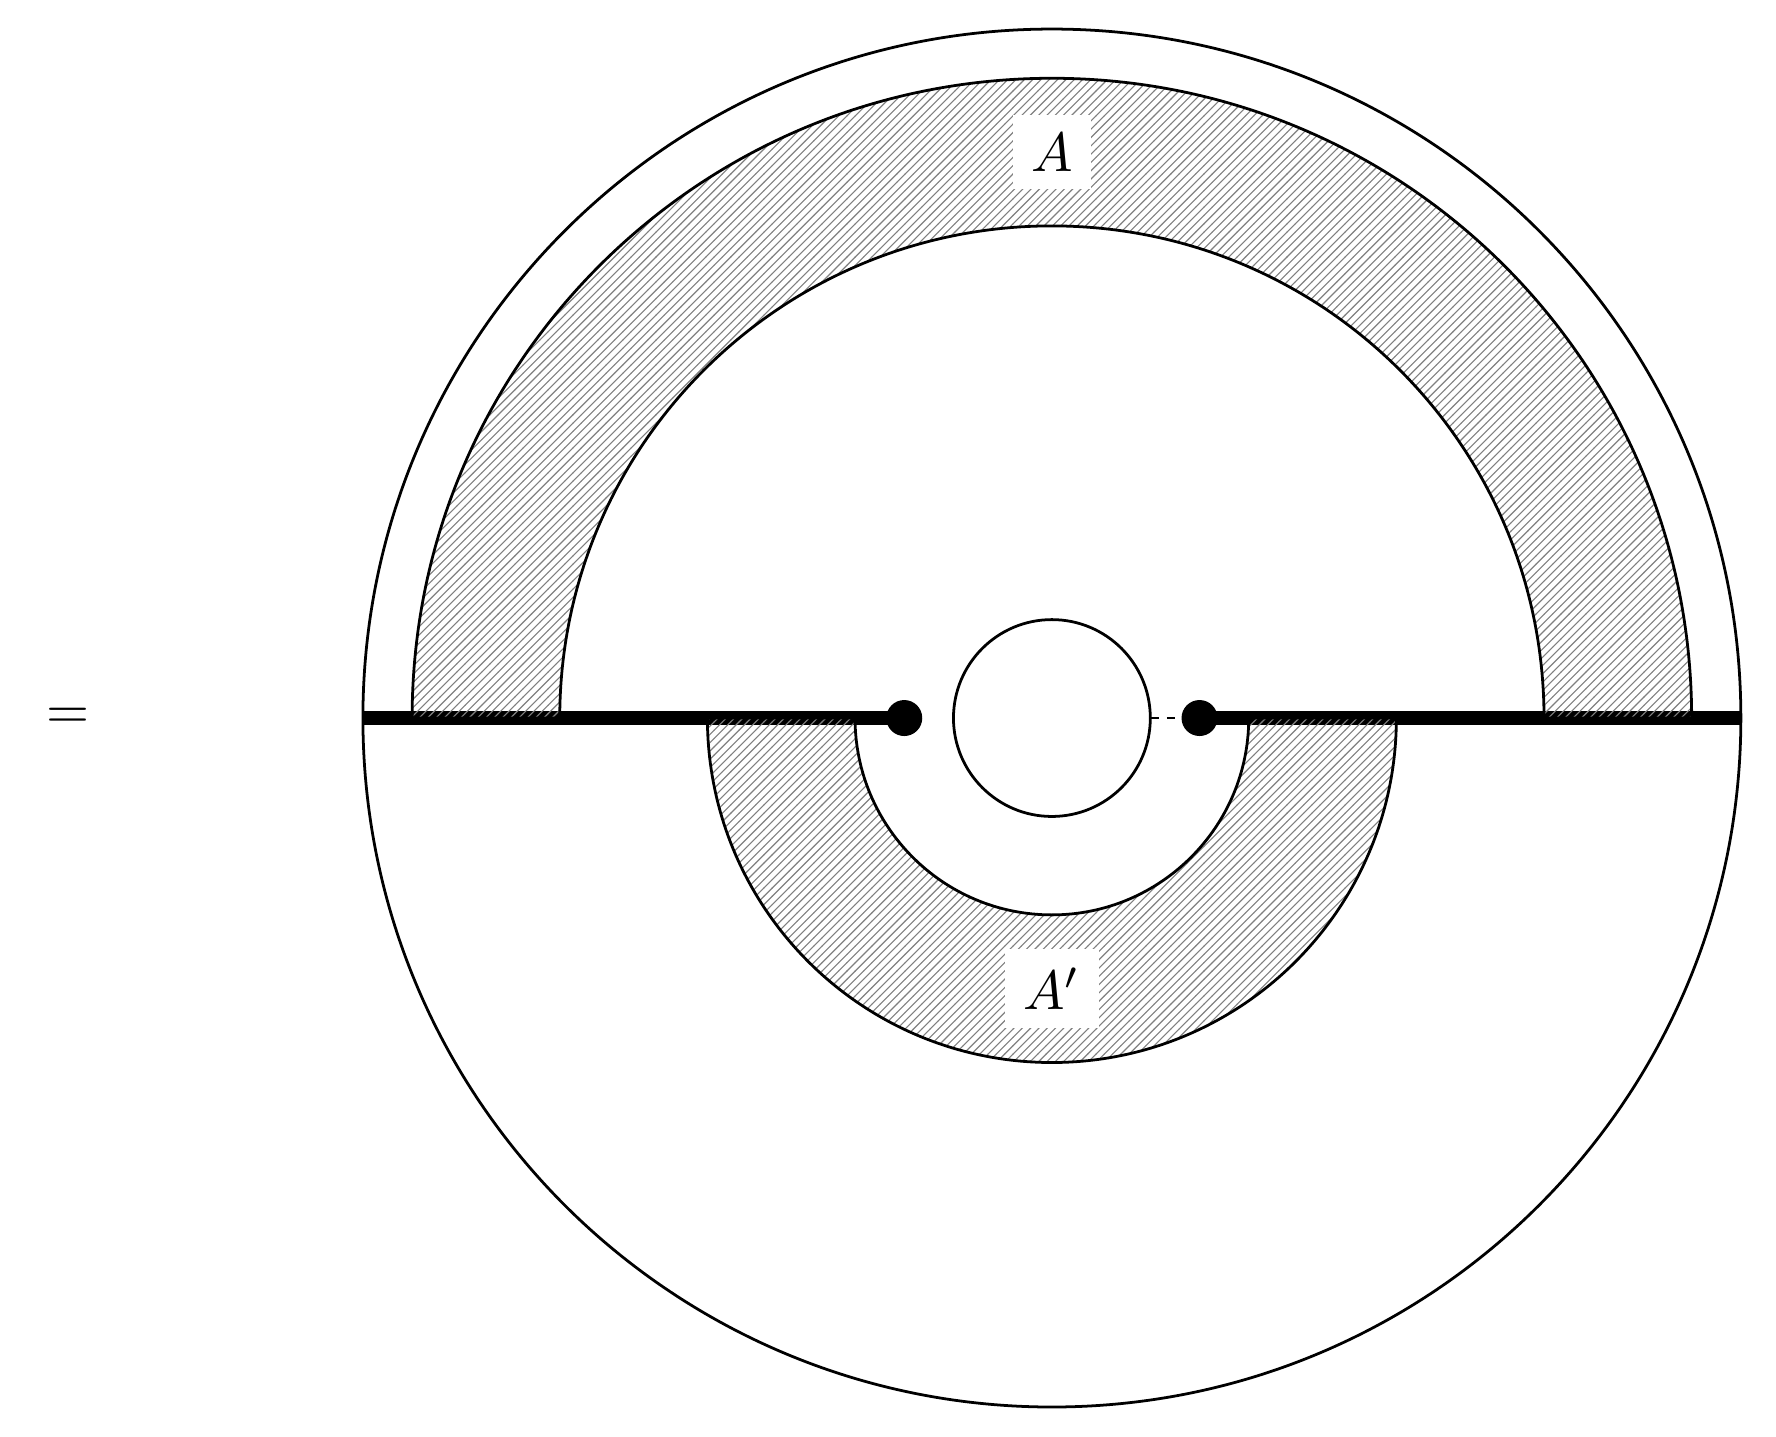
\begin{tikzpicture}[x=1.25cm, y=1.25cm, line width=1pt]

% draw '='
\node[scale = 2] at (-10, 0) {$=$};

% draw inner and outer circle
\draw[color=black] (0, 0) circle (1);
\draw[color=black] (0, 0) circle (7);

% draw 0 line
\draw[dashed] (0 : 1) -- ( 0: 7);

% draw slits
\draw[color=black, line width=5pt] (0 : 1.5) -- (0 : 7);
\draw[color=black, line width=5pt] (180 : 1.5) -- (180 : 7);
\filldraw (0 : 1.5) circle (6pt);
\filldraw (180 : 1.5) circle (6pt);

% draw shaded concentrical stripes
\filldraw[pattern=north east lines, pattern color=black!50] (180 : 5) arc [radius = 5, start angle = 180, delta angle = -180]
                                                     -- (0 : 6.5) arc [radius = 6.5, start angle = 0, delta angle = 180]
                                                     -- cycle;
\filldraw[pattern=north east lines, pattern color=black!50] (0 : 3.5) arc [radius = 3.5, start angle = 0, delta angle = -180]
                                                     -- (180 : 2) arc [radius = 2, start angle = 180, delta angle = 180]
                                                     -- cycle;

% draw labels
\node[scale = 2, fill = white] at (90 : 5.75) {$A$};
\node[scale = 2, fill = white] at (270 : 2.75) {$A'$};

\end{tikzpicture}
}
\end{document}